\section{Results}
\label{sec:results}
We evaluate the method presented in 3 similar \emph{Suzanne} scenes, differing in the shapes of the portal and the light (\ref{fig:results}). 

\begin{itemize}
\item Scene \autoref{img:results_small} has a small portal with a comparatively large source behind it. The monkey is in the monkey is then in the antiantumbra of the portal, making uniform portal sampling the best approach.

\item Scene \autoref{img:results_big} has a large portal with a small light behind it. The monkey is in the antiumbra, making Light sampling the optimal approach.

\item Scene \autoref{img:results_balanced} has a similarly sized light and portal, arranged so that they don't fully overlap. The monkey is then located in the antipenumbra, making projection sampling optimal.
\end{itemize}

For each scene, we compare against the four sampling approaches presented in the paper. Each sampling strategy is then combined with BSDF sampling using MIS.

\begin{itemize}
    \item \textbf{Light (baseline):} Sampling the target lights area uniformly.
    \item \textbf{Portal:} Sampling the portal area uniformly .
    \item \textbf{Projection:} Sampling the lights projection onto the portal.
    \item \textbf{Antishadow:} First we determine in which region of the portal's antishadow the shading point resides in, then choose the least expensive, optimal strategy from the above three.
\end{itemize}

We provide the measured MSE over time for each sampling strategy. The results indicate that light and portal sampling are not robust as each strategy only works well in one of the three scenes. Projection is robust as it works adequately in all scenes, but at a minor runtime overhead, due to projecting and clipping the portal. Lastly, antishadow-based sampling gives the best of both worlds, as it works well in all scenes and has a lower runtime overhead than projection sampling.

\begin{figure*}[ht]
    \centering
    \subfloat[\textbf{Large light, small portal:} Optimal sampling strategy is portal.]{
        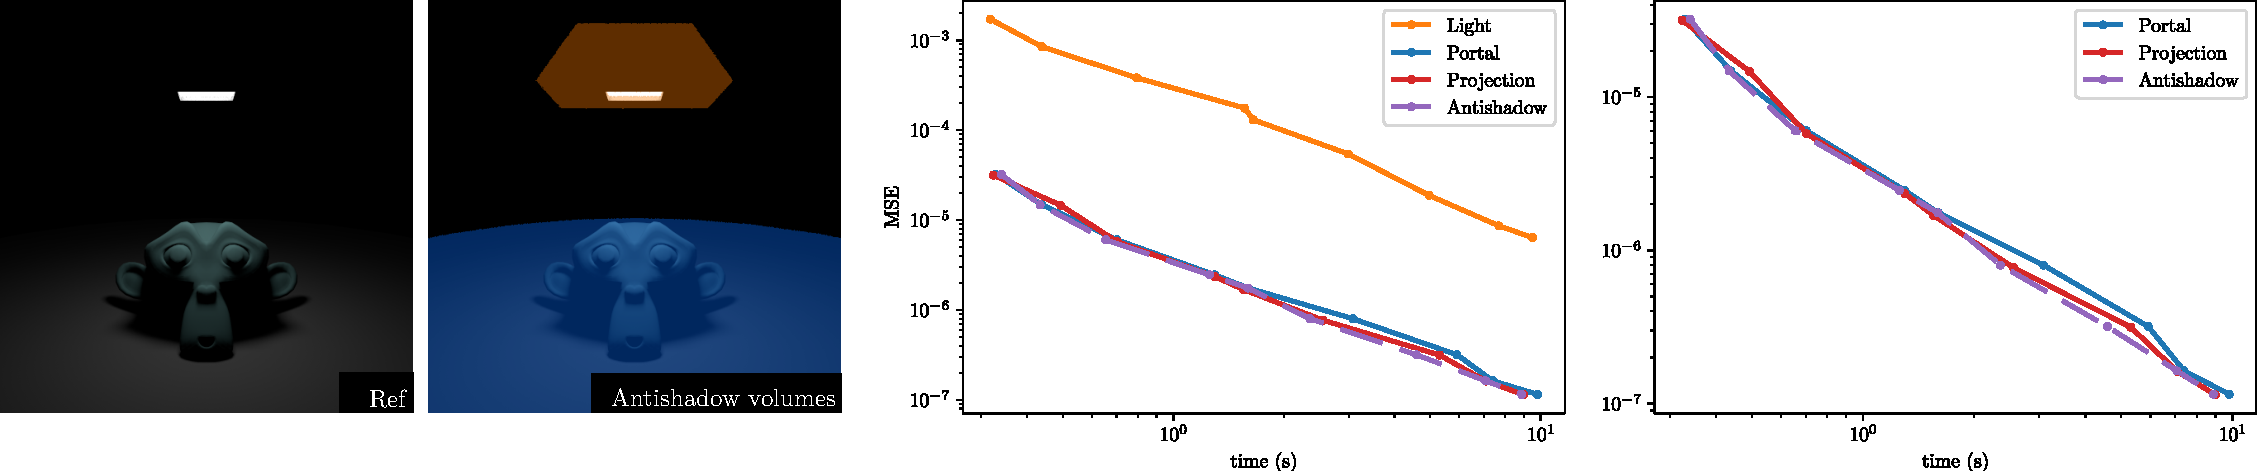
\includegraphics[width=\textwidth]{../pdf/results_a.pdf}
        \label{img:results_small}
    }
    
    \subfloat[\textbf{Small light, large portal:} Optimal sampling strategy is projection.]{
        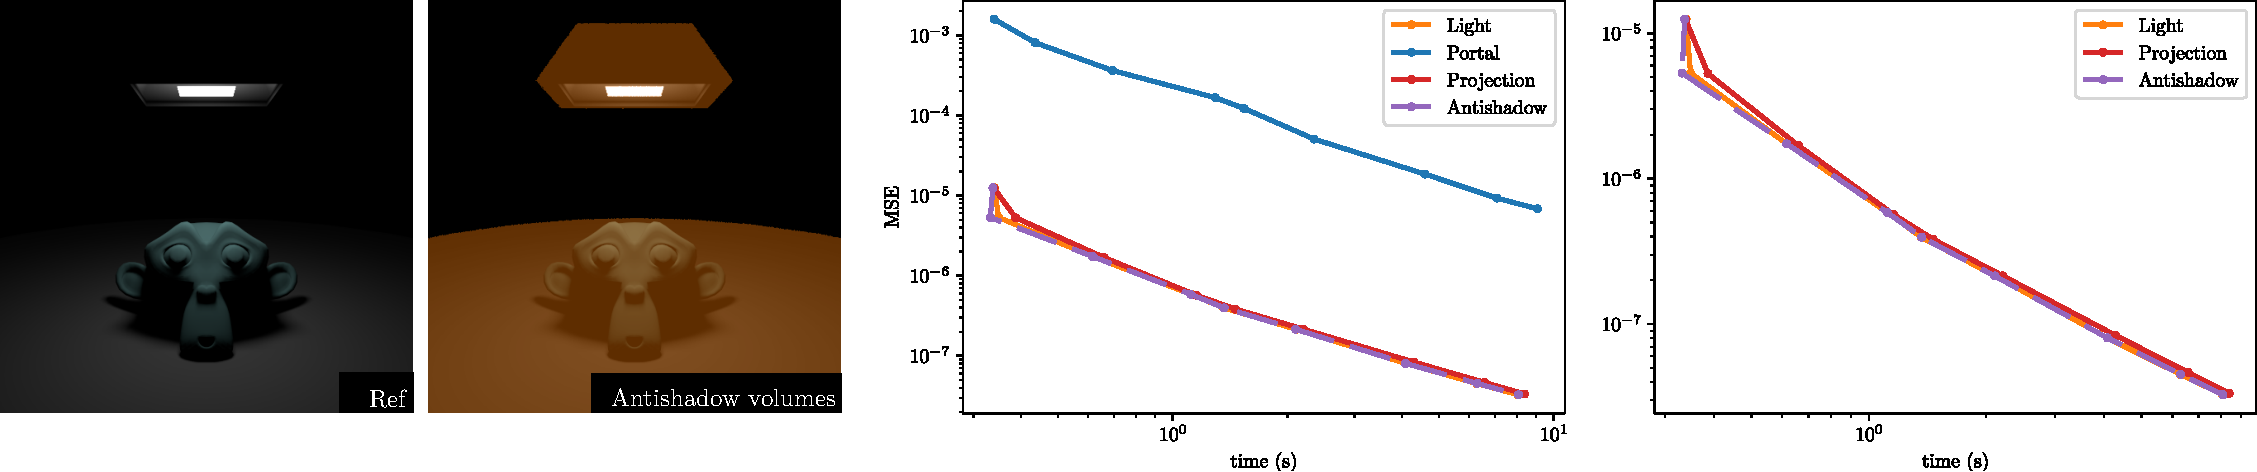
\includegraphics[width=\textwidth]{../pdf/results_b.pdf}
        \label{img:results_big}
    }
    
    \subfloat[\textbf{Balanced light and portal:} Optimal sampling strategy is projection.]{
        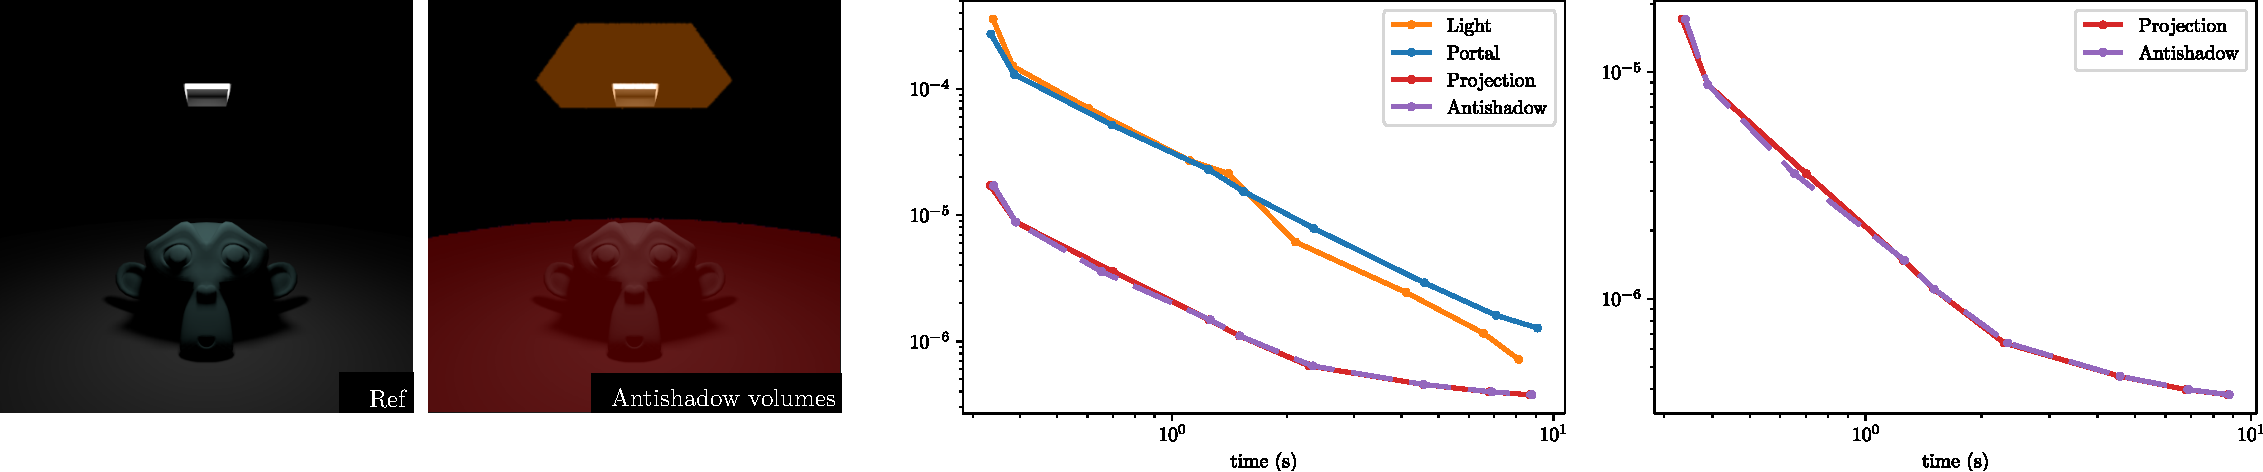
\includegraphics[width=\textwidth]{../pdf/results_c.pdf}
        \label{img:results_balanced}
    }

    \caption{We compare light sampling (baseline), portal sampling, projection sampling and antishadow-based sampling for three \emph{Suzanne} scenes, differing in the portal-light solid angle ratios. Light and portal sampling are not robust as they fail in all scenes but one. Projection sampling works well in all scenes at a small runtime cost, and antishadow-based sampling works as well as projection sampling but at a decreased runtime cost.}
    \label{fig:results}
\end{figure*}


